\scanpage{207}
\uline{Faisons varier} $x$ pt complexe (ou place ``archimédienne''). Je pense que \uline{les}
$\xi_{x,\mathbf Z}$ \uline{et même les} $\xi_{x,\mathbf R}$ \inserted{[$\simeq\xi_{x,\mathbf C}$ muni de $\tau$]}
\uline{qui correspondent à des places distinctes sont non isomorphes}.

\margin{\figure{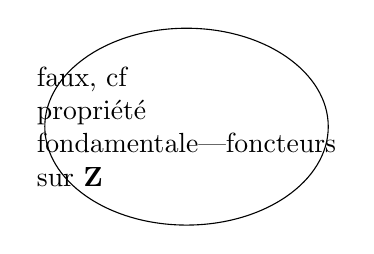
\begin{tikzpicture}
\draw (0,0) ellipse (1.8 and 1.25);
\node[align=left] at (0,0) {faux, cf\\\unsure{propriété}\\\unsure{fondamentale|foncteurs}\\sur $\mathbf Z$};
\end{tikzpicture}}}

Quant aux $\xi_{x,\mathbf C}=\xi_{x,\infty}$, eux \unsure{ms}
\deleted{\unsure{puisque}}\inserted{comme $k$ est}
\deleted{\unsure{nous avons dit}, ils sont}
alg. clos ils sont isomorphes entre eux, mais pas canoniquement ....

\uline{NB} En car $p>0$, je pense que $T_\alpha(\mathbf R)=\varnothing$
en général, ce qui explique qu'il n'y ait pas de phénomènes de
``composantes connexes'' ``Ramification en $\mathbf R$'' ...
à considérer alors ...

\margin{\unsure{s'éclaircir si} il ne peut y avoir des pt à val. dans une ext. tot. réelle ???}

Si

\figure{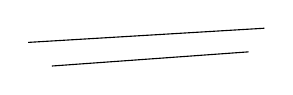
\begin{tikzpicture}\draw (0,0)--(3,.18);\draw (.3,-.3)--(2.8,-.12);\end{tikzpicture}}

Pt motivique de $X$ à valeurs dans un corps (ou un anneau) $k$: objet de $T(k)$.
Langage de la \uline{fibre d'un motif en un point}.
Les pts forment une catégorie fibrée sur $(\mathrm{Sch})$, munie de fpqc,
\deleted{\unsure{elle}} c'est un \uline{torseur}.
Pour $k$ donné, les isom. d'un \deleted{objet} $\xi\in T(k)$ sur un autre forment le

\margin{206}
